\documentclass{article}
\oddsidemargin=0cm
\topmargin=-1cm
\textwidth=16cm
\textheight=25cm
\usepackage{graphicx}          % include graphics
\usepackage{array}
\newcolumntype{L}[1]{>{\raggedright\let\newline\\\arraybackslash\hspace{0pt}}m{#1}}
\newcolumntype{C}[1]{>{\centering\let\newline\\\arraybackslash\hspace{0pt}}m{#1}}
\newcolumntype{R}[1]{>{\raggedleft\let\newline\\\arraybackslash\hspace{0pt}}m{#1}}


\usepackage[most]{tcolorbox}
\newcounter{bmcsexample}
\usepackage{xparse}
\usepackage{lipsum}

\def\exampletext{Example} % If English

\NewDocumentEnvironment{bmcsexample}{ O{} }
{
\colorlet{colexam}{red!55!black} % Global example color
\newtcolorbox[use counter=bmcsexample]{bmcsexamplebox}{%
    % Example Frame Start
    empty,% Empty previously set parameters
    title={\exampletext: #1},% use \thetcbcounter to access the bmcsexample counter text
    % Attaching a box requires an overlay
    attach boxed title to top left,
       % Ensures proper line breaking in longer titles
       minipage boxed title,
    % (boxed title style requires an overlay)
    boxed title style={empty,size=minimal,toprule=0pt,top=4pt,left=3mm,overlay={}},
    coltitle=colexam,fonttitle=\bfseries,
    before=\par\medskip\noindent,parbox=false,boxsep=0pt,left=3mm,right=0mm,top=2pt,breakable,pad at break=0mm,
       before upper=\csname @totalleftmargin\endcsname0pt, % Use instead of parbox=true. This ensures parskip is inherited by box.
    % Handles box when it exists on one page only
    overlay unbroken={\draw[colexam,line width=.5pt] ([xshift=-0pt]title.north west) -- ([xshift=-0pt]frame.south west); },
    % Handles multipage box: first page
    overlay first={\draw[colexam,line width=.5pt] ([xshift=-0pt]title.north west) -- ([xshift=-0pt]frame.south west); },
    % Handles multipage box: middle page
    overlay middle={\draw[colexam,line width=.5pt] ([xshift=-0pt]frame.north west) -- ([xshift=-0pt]frame.south west); },
    % Handles multipage box: last page
    overlay last={\draw[colexam,line width=.5pt] ([xshift=-0pt]frame.north west) -- ([xshift=-0pt]frame.south west); },%
    }
\begin{bmcsexamplebox}}
{\end{bmcsexamplebox}\endlist}


\begin{document}
        
\begin{bmcsexample}[Bond damage and plasticity]
\noindent This example shows the response of bond material point 
which enters simultaneously the yielding and damage regime. Damage is 
increasing during the first loading branch. Subsequently, the exhibits
material point exhibits kinematic hardening upon unloading and reloading.
 \\[3mm]
\begin{center}
\begin{tabular}{lrp{4cm}}\hline
Model parameter & Symbol = Value [Unit] & Description  \\\hline \hline
n\_steps & $n_\mathrm{s}$ = 100 [-] & {\footnotesize None}  \\
            material\_model & option = damage-plasticity [-] & {\footnotesize None}  \\
            interaction\_type & option = predefined [-] & {\footnotesize None}  \\
            \hline
\multicolumn{3}{l}{loading\_scenario : LoadingScenario}\\ \hline

number\_of\_cycles & $n_\mathrm{cycles}$ = 3 [-] & {\footnotesize None}  \\
            number\_of\_increments & $n_{\mathrm{incr}}$ = 20 [-] & {\footnotesize None}  \\
            loading\_type & option = cyclic [-] & {\footnotesize None}  \\
            maximum\_loading & $\phi_{\max}$ = 0.003 [-] & {\footnotesize None}  \\
            amplitude\_type & option = constant [-] & {\footnotesize None}  \\
            unloading\_ratio & $\phi_{\mathrm{unload}}$ = 0.8 [-] & {\footnotesize None}  \\
            loading\_range & option = symmetric [-] & {\footnotesize None}  \\
            
\multicolumn{3}{r}{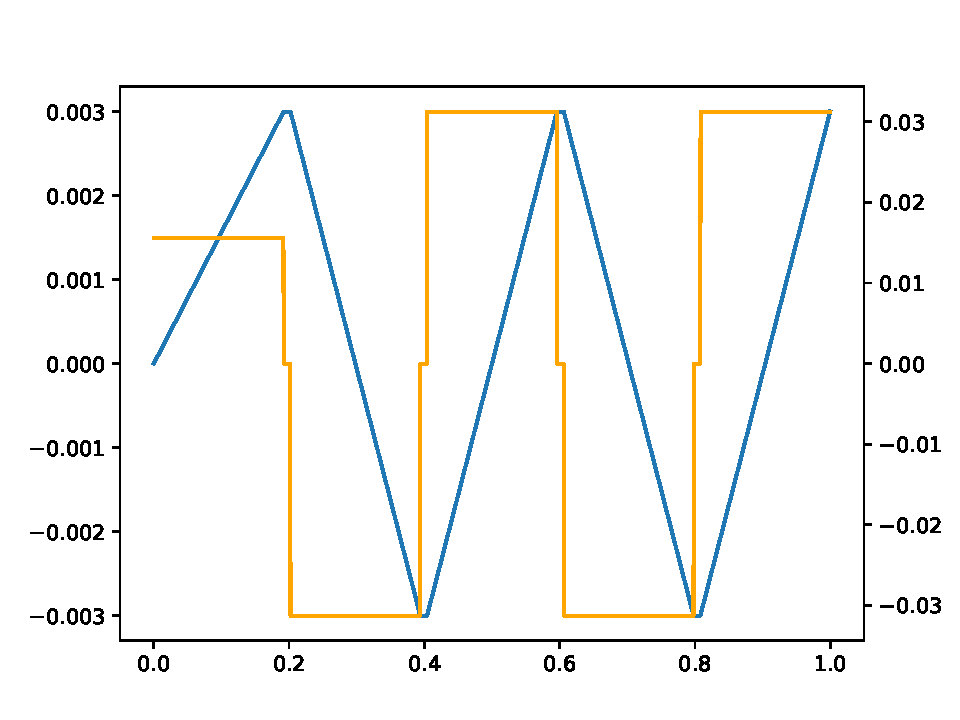
\includegraphics[width=5cm]{fig140677184635824.pdf}}\\
\hline
\multicolumn{3}{l}{mats\_eval : MATSBondSlipDP}\\ \hline

E\_b & $E_\mathrm{b}$ = 12900 [MPa/mm] & {\footnotesize Bond stiffness}  \\
            K & $K$ = 1000.0 [MPa/mm] & {\footnotesize Isotropic hardening modulus}  \\
            tau\_bar & $\bar{\tau}$ = 5 [MPa] & {\footnotesize Yield stress}  \\
            omega\_fn\_type & None = li [None] & {\footnotesize None}  \\
            gamma & $\gamma$ = 0.0 [MPa/mm] & {\footnotesize Kinematic hardening modulus}  \\
            \hline
\multicolumn{3}{l}{omega\_fn : LiDamageFn}\\ \hline

s\_0 & $s_0$ = 0.0004 [None] & {\footnotesize elastic strain limit}  \\
            alpha\_2 & $\alpha_2$ = 2000.0 [None] & {\footnotesize parameter controls the damage function}  \\
            alpha\_1 & $\alpha_1$ = 1.0 [None] & {\footnotesize parameter controls the damage function}  \\
            
\multicolumn{3}{r}{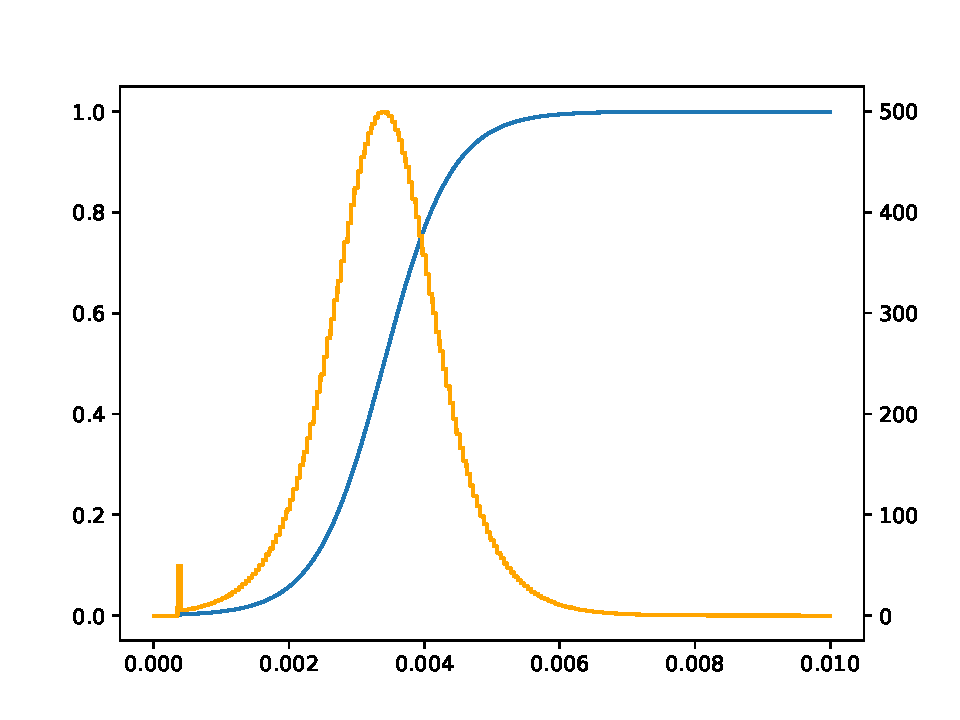
\includegraphics[width=5cm]{fig140675832007280.pdf}}\\
\hline \end{tabular}


\end{center}

\noindent
\begin{tabular}{L{7.5cm}L{7.5cm}}
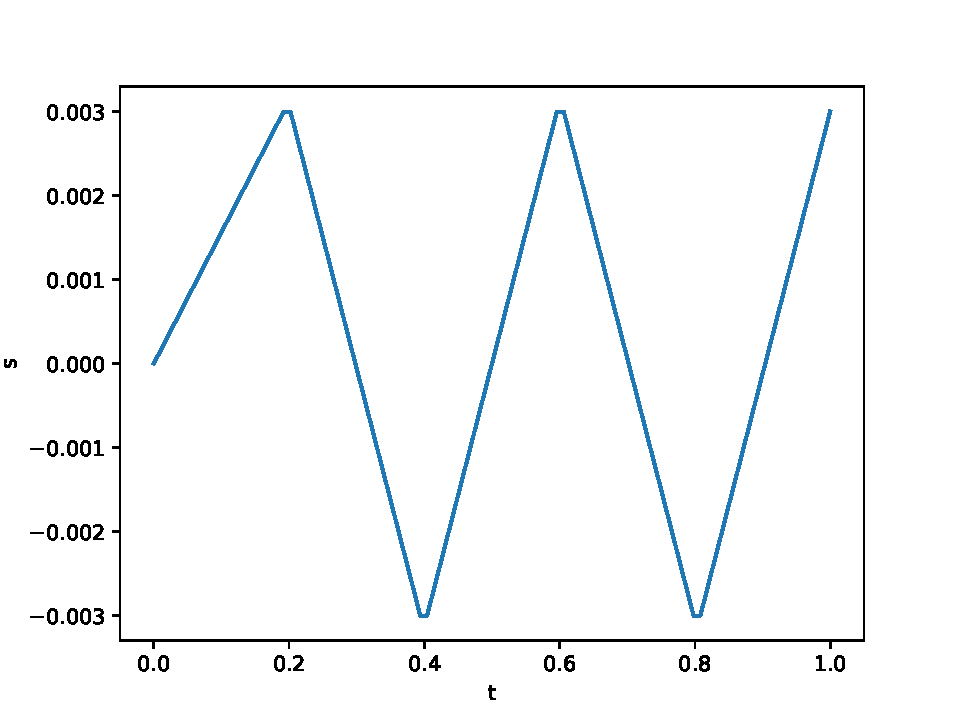
\includegraphics[width=7.5cm]{fig140675832832464.pdf}
 & 
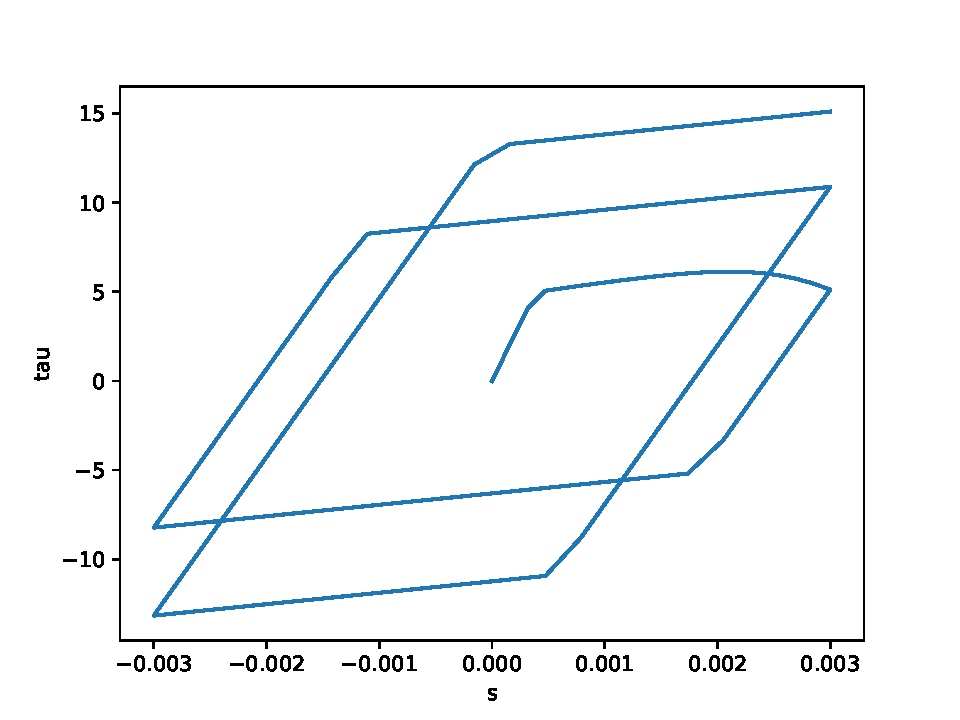
\includegraphics[width=7.5cm]{fig140675827491088.pdf}
 \\\end{tabular}

\noindent
\begin{tabular}{L{7.5cm}L{7.5cm}}
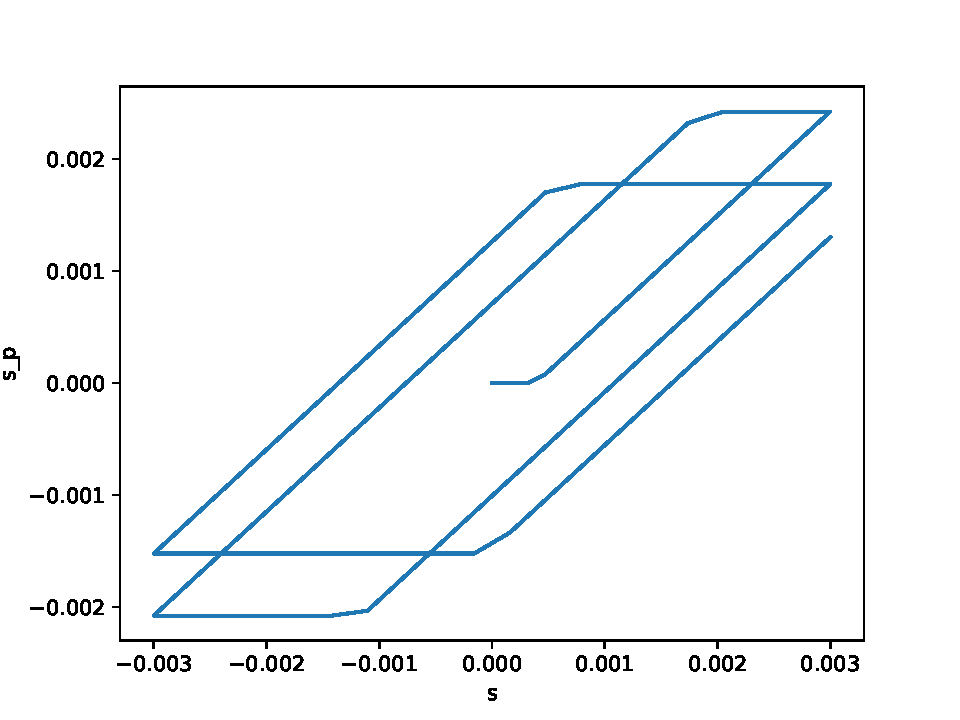
\includegraphics[width=7.5cm]{fig140675827491664.pdf}
 & 
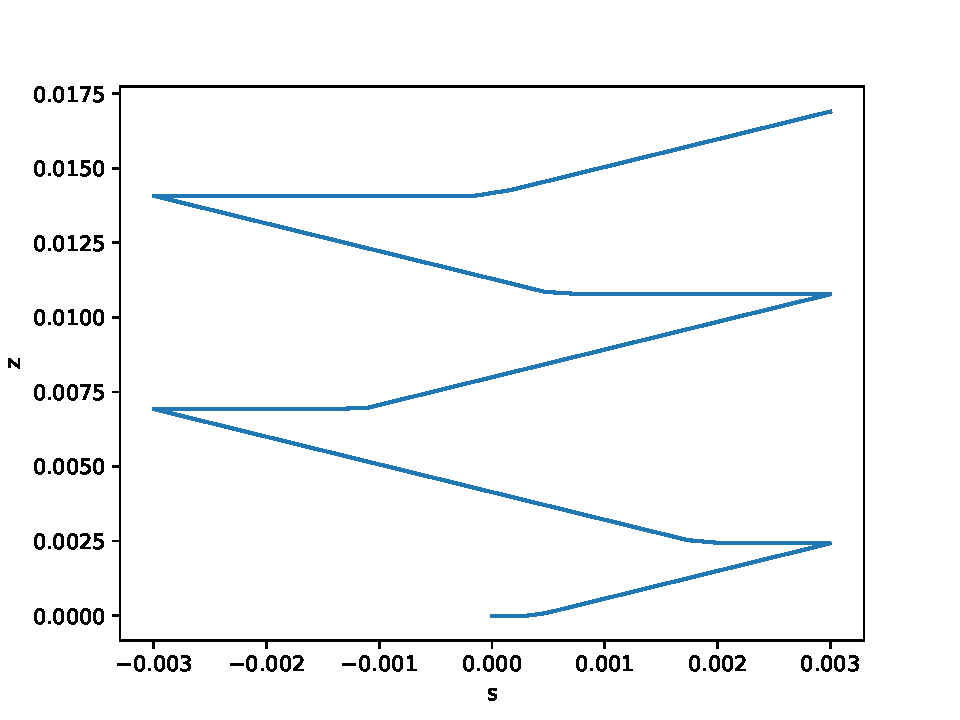
\includegraphics[width=7.5cm]{fig140675827492144.pdf}
 \\\end{tabular}

\noindent
\begin{tabular}{L{7.5cm}L{7.5cm}}
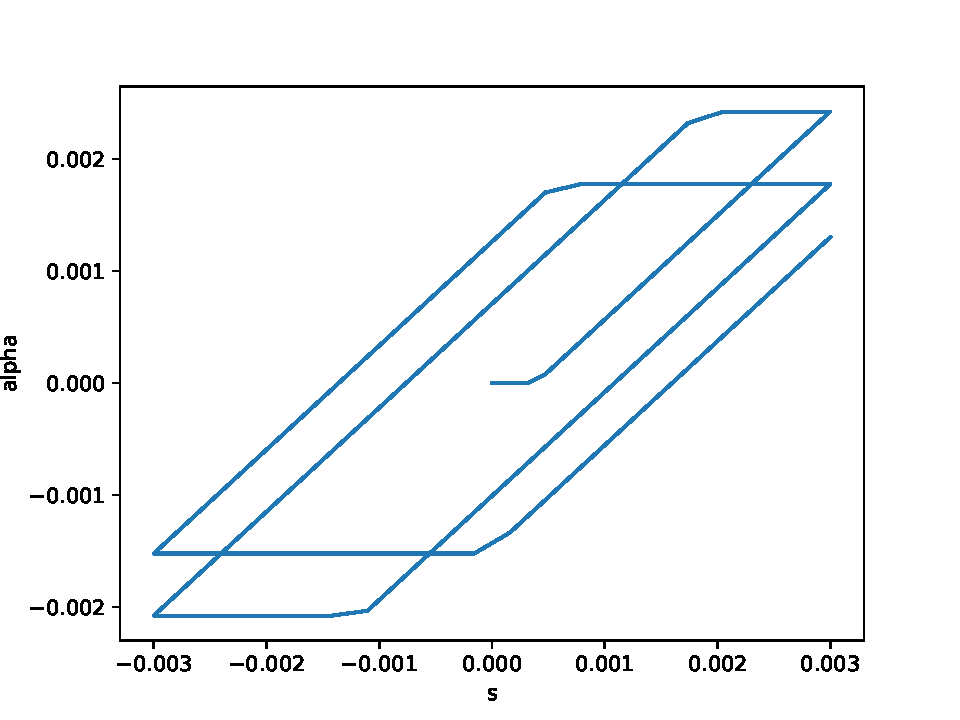
\includegraphics[width=7.5cm]{fig140675827492624.pdf}
 & 
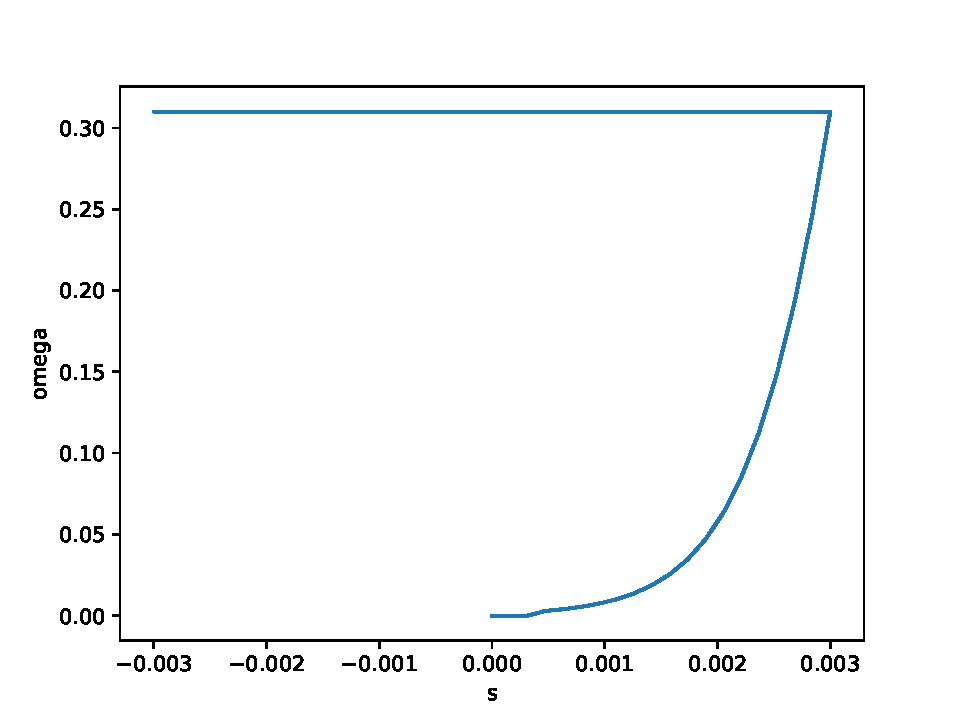
\includegraphics[width=7.5cm]{fig140675827493104.pdf}
 \\\end{tabular}

\end{bmcsexample}

\end{document}
        